  \newpage
  \subsection{Create a new run}
Every User can create a new run, specifying the start and finish locations, date, time and the maximum number of enrollments.

\begin{table}[H]
	\centering
    
    \begin{tabular}{|p{3.5cm}|p{10.3cm}|}
    
    \hline
    \textbf{\large{Actors}} & Organizer \\			
    \hline		 					
    \textbf{\large{Goals}} 				& \ref{goal:run1}\\
    
    \hline
    \textbf{\large{Enter Condition}}	& The Organizer is already logged in.		\\
    
    \hline
    \textbf{\large{Events Flow}}		& \begin{enumerate}[leftmargin=0.5cm]
                                          	\item The \emph{Organizer} accesses the "Create Run" page of the application.
                                            \item The \emph{Organizer} inserts all the required information to define the run (start and finish locations, date, time and maximum number of participants).
                                             \item The \emph{Organizer} defines the list of intermediate locations that will be part of the run's path (optional)
                                            \item The System adds the new run to the list of scheduled runs.
                                           
                                          \end{enumerate}
    										\\
    \hline
    \textbf{\large{Exit Conditions}}    & The new run is created and successfully added to the list of scheduled runs.  \\
    
    \hline
    \textbf{\large{Exceptions}} 		& \begin{enumerate}[leftmargin=0.5cm]
    	\item The \emph{Organizer} specified points that are not reachable on foot.
	\item The \emph{Organizer} specified a negative maximum number of participants.
	\item The \emph{Organizer} specified a date or time which belongs to the past.                                        	\item The \emph{Organizer} specified a run with all the same informations of another run.
	\end{enumerate}
	
If one of these problems occur, the system shows an error message to the user, which is invited to insert the required information again.\\
    
    \hline
    
    \end{tabular}
	
\end{table}

\begin{figure}[H]
    \centering
    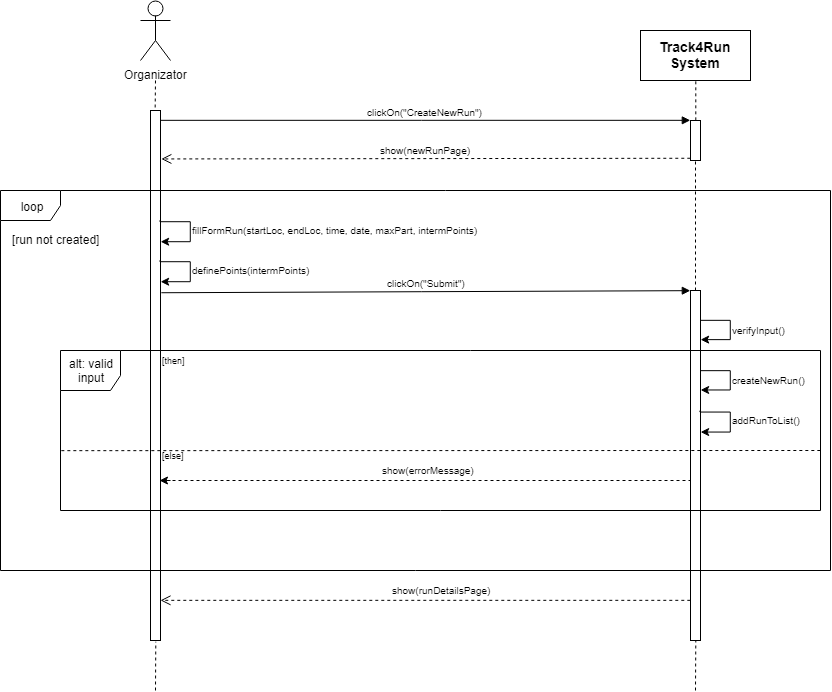
\includegraphics[scale=0.4]{Pictures/createNewRunSeqDiag.png}
    \caption{Sequence diagram for creating a new run}
\end{figure}
